%%%%%%%%%%%%%%%%%%%%%%%%%%%%%%%%%%%%%%%%%
% Journal Article
% LaTeX Template
% Version 1.3 (9/9/13)
%
% This template has been downloaded from:
% http://www.LaTeXTemplates.com
%
% Original author:
% Frits Wenneker (http://www.howtotex.com)
%
% License:
% CC BY-NC-SA 3.0 (http://creativecommons.org/licenses/by-nc-sa/3.0/)
%
%%%%%%%%%%%%%%%%%%%%%%%%%%%%%%%%%%%%%%%%%

%----------------------------------------------------------------------------------------
%	PACKAGES AND OTHER DOCUMENT CONFIGURATIONS
%----------------------------------------------------------------------------------------

\documentclass[twoside]{article}

%\documentclass{aastex}  % version 5.0 or prior
%\usepackage{natbib}



\usepackage{graphicx}
\usepackage{lipsum} % Package to generate dummy text throughout this template

\usepackage[sc]{mathpazo} % Use the Palatino font
\usepackage[T1]{fontenc} % Use 8-bit encoding that has 256 glyphs
\linespread{1.05} % Line spacing - Palatino needs more space between lines
\usepackage{microtype} % Slightly tweak font spacing for aesthetics

\usepackage[hmarginratio=1:1,top=32mm,columnsep=20pt]{geometry} % Document margins
\usepackage{multicol} % Used for the two-column layout of the document
\usepackage[hang, small,labelfont=bf,up,textfont=it,up]{caption} % Custom captions under/above floats in tables or figures
\usepackage{booktabs} % Horizontal rules in tables
\usepackage{float} % Required for tables and figures in the multi-column environment - they need to be placed in specific locations with the [H] (e.g. \begin{table}[H])
\usepackage{hyperref} % For hyperlinks in the PDF
\usepackage{subcaption}

\usepackage{lettrine} % The lettrine is the first enlarged letter at the beginning of the text
\usepackage{paralist} % Used for the compactitem environment which makes bullet points with less space between them
\usepackage{amsmath}
\usepackage{abstract} % Allows abstract customization
\renewcommand{\abstractnamefont}{\normalfont\bfseries} % Set the "Abstract" text to bold
\renewcommand{\abstracttextfont}{\normalfont\small\itshape} % Set the abstract itself to small italic text

\usepackage{titlesec} % Allows customization of titles
\renewcommand\thesection{\Roman{section}} % Roman numerals for the sections
\renewcommand\thesubsection{\Roman{subsection}} % Roman numerals for subsections
\renewcommand\thesubsubsection{\Alph{subsubsection}} % Roman numerals for subsections
\titleformat{\section}[block]{\large\scshape\centering}{\thesection.}{1em}{} % Change the look of the section titles
\titleformat{\subsection}[block]{\large}{\thesubsection.}{1em}{} % Change the look of the section titles
\titleformat{\subsubsection}[block]{}{\thesubsubsection.}{1em}{} % Change the look of the section titles

\usepackage{fancyhdr} % Headers and footers
\pagestyle{fancy} % All pages have headers and footers
\fancyhead{} % Blank out the default header
\fancyfoot{} % Blank out the default footer
\fancyhead[C]{PHSX567 Final Project Report $\bullet$ \today } % Custom header text
\fancyfoot[RO,LE]{\thepage} % Custom footer text


%----------------------------------------------------------------------------------------
%	TITLE SECTION
%----------------------------------------------------------------------------------------

\title{\vspace{-15mm}\fontsize{24pt}{10pt}\selectfont\textbf{MOSES Data Inversion With Convolutional Neural Networks}} % Article title

\author{
\large
\textsc{Roy Smart}\\[2mm] % Your name
\normalsize Montana State University \\ % Your institution
\normalsize \href{mailto:roy.smart@montana.edu}{roytsmart@gmail.com} % Your email address
\vspace{-5mm}
}
\date{}

%----------------------------------------------------------------------------------------

\begin{document}

\maketitle % Insert title

\thispagestyle{fancy} % All pages have headers and footers

%\begin{abstract}
%We present a novel way of performing MOSES data inversions using a
%\end{abstract}

%----------------------------------------------------------------------------------------
%	ARTICLE CONTENTS
%----------------------------------------------------------------------------------------

\begin{multicols}{2} % Two-column layout throughout the main article text

\section{Introduction}
\lettrine{T}{he} \textit{Multi-Order Solar EUV Spectrograph} (MOSES) is a unique instrument developed by Charles Kankelborg's research group at Montana State University that captures solar images in three diffraction orders: $m=0,+1,$ and $-1$. Unlike most spectrographs, MOSES is not equipped with a slit to restrict the field of view on the dispersion axis. The advantage of this configuration is that the instrument simultaneously views spatial-spectral information, allowing interesting solar features to be more easily identified. However this lack of spatial restriction by a slit means that spectral and spatial information are convolved together to form the images captured by MOSES. These images are known as \textit{overlappograms}. \par
\begin{figure}[H]
	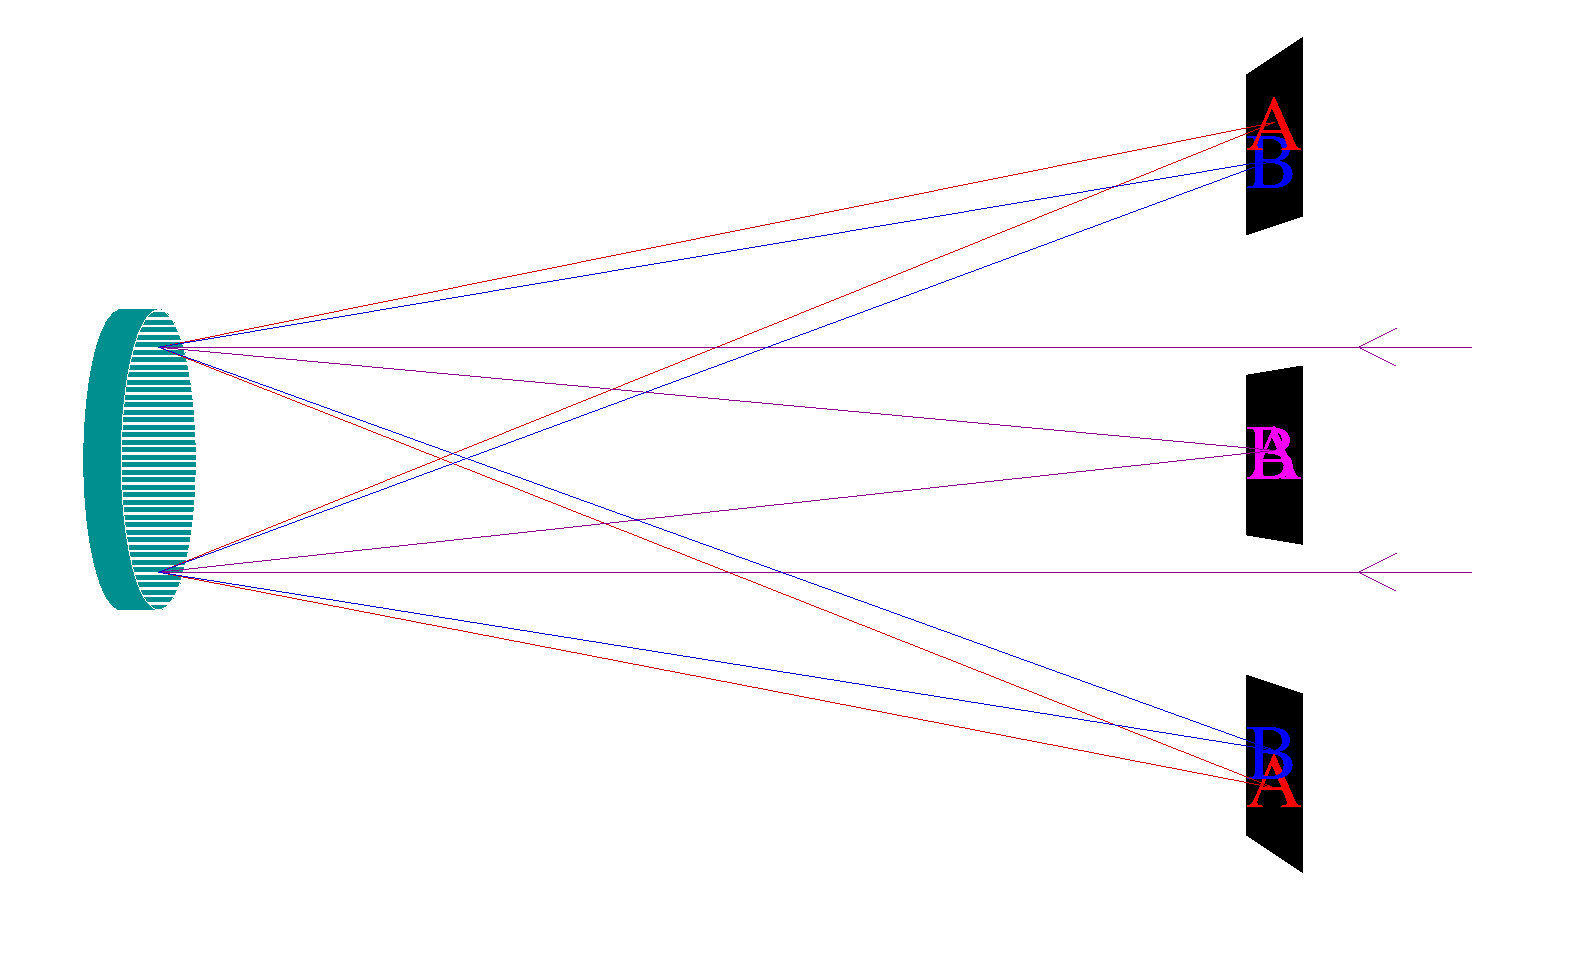
\includegraphics[width=\linewidth]{images/instrument.eps}
	\caption{Layout of the MOSES instrument demonstrating how different wavelengths are overlapped onto each detector \cite{moses}.}
\end{figure}
The main objective of the MOSES instrument is to determine Doppler shifts of the structures observed in the solar transition region. To find this quantity, we must perform what we call an \textit{inversion}. This is best described as taking the 2-dimensional spectral and spatial information from each of the three detectors and constructing a spectral \textit{cube} in three dimensions, with two spatial dimensions and one spectral dimension.
\begin{figure}[H]
	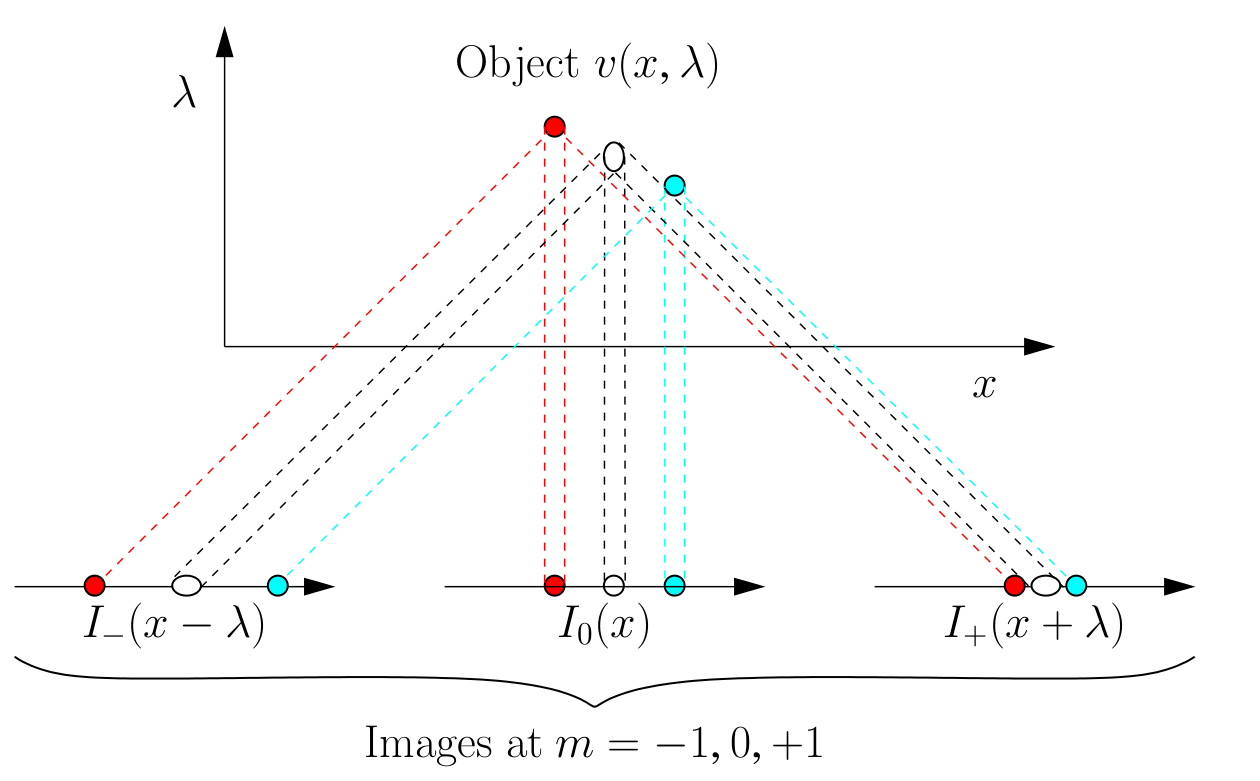
\includegraphics[width=\linewidth]{images/inversion}
	\caption{Diagram demonstrating how compact objects in the data cube are convolved to form the images at each detector \cite{moses}.}
	\label{inversion}
\end{figure}
The main challenge with inverting the MOSES data is that it is an obviously ill-posed problem, i.e. the spectral cube contains more information than is provided by the instrument. This is mathematically described using the expression
\begin{equation}
I_m(x',y') = \int_B v(x'-m \lambda,y',\lambda)d\lambda. \label{invert}
\end{equation}
Where $I(x',y')$ is the intensity measured by the instrument, $v(x',y',\lambda)$ is an object located in the spectral cube, $m$ is the spectral order, $(x',y')$ are the detector coordinates, and the domain $B$ is the passband of the instrument. 
\par Since Equation \eqref{invert} doesn't have a unique solution, there are many possible cubes that could produce the same images captured by MOSES. Consequently, we must use physical constraints to attempt to trim down the large number of potential solutions to the inversion problem. \par 

\section{Motivation}

Many researchers throughout the history of the MOSES research project have developed computational tools to solve the inversion problem. These methods include Smoothed Multiplicative Algebraic Reconstruction Technique (SMART)\cite{smart}, Fourier backprojection and pixon inversion \cite{inversion} and are discussed in detail in the literature. 
\par The above methods have proved successful in revealing the interior structure of the transition region \cite{moses}. However there is still room for progress toward full inversions of the entire MOSES dataset. These algorithms have a tendency to produce what is known as \textit{plaid}. This is a phenomenon where bright objects on the spectral cube tend to be smeared across the direction of the spectral projections, producing decidedly unphysical inversions.

\begin{figure}[H]
	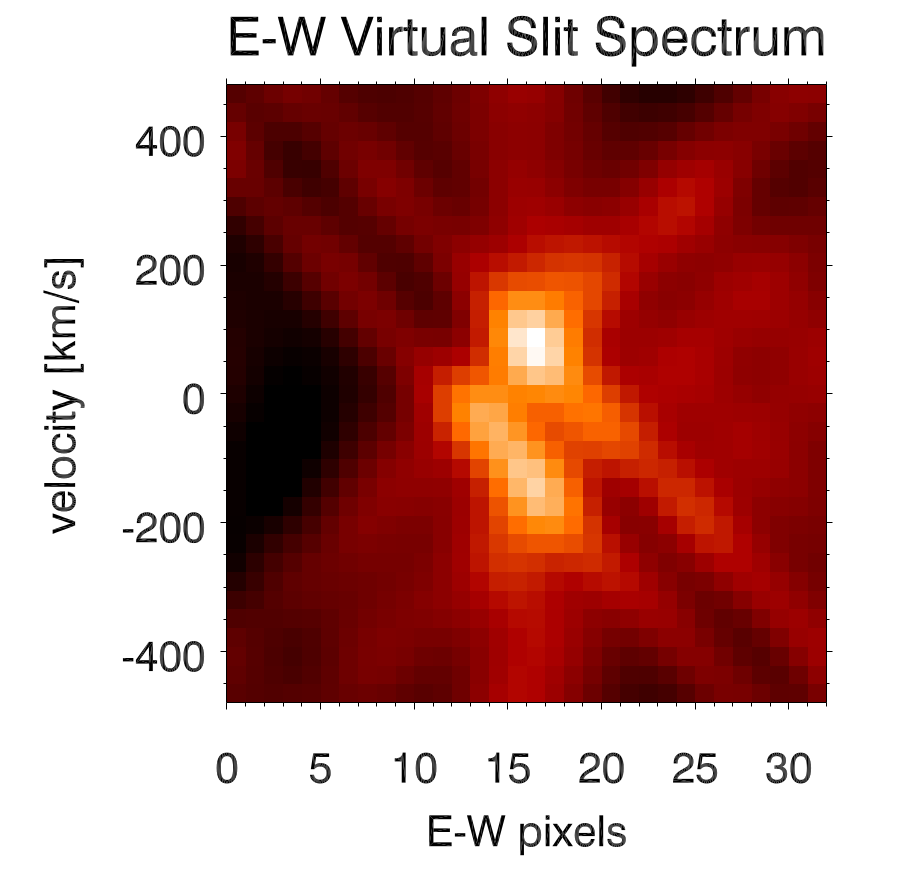
\includegraphics[width=\linewidth]{images/plaid2}
	\caption{An example of plaid. Notice how the bright pixels in the center are smeared diagonally (projection dimension) across the image. This is an example of an unphysical inversion. \cite{tom} }
\end{figure} 

Developing an inversion method that is resistant to plaid would be very beneficial, as such an inversion would allow researchers to extract more scientific information about the structure of the transition region.

\section{Proposed Inversion Method}
\subsection{Machine Learning}
Thus far, all of the attempts to invert the MOSES data have relied on traditional, human-designed algorithms to carry out the computation. However, in the past few years, great strides have been made in machine learning, where a computer program is trained to solve a particular problem by providing examples of the problem along with each corresponding solution. Feedback is then provided to the network so that it may utilize minimization techniques to converge on a solution. \par We propose that a method based off of machine learning might allow some progress to be made toward the goal of plaid-resistant MOSES inversions. This is made possible by the fact that the learning algorithm could be penalized for producing plaid solutions to the inversion problem and rewarded for producing physical solutions.  \par While machine learning sounds like a fantastic approach to problem solving, there is still a great deal of challenges to with which to contend. First, the structure of the learning algorithm is very important in determining its problem-solving ability and, unlike traditional algorithms, the right structure can often only be found by trial and error. Furthermore, the learning process takes a large number of examples to converge on the solution. Solving these problems will be discussed in the following pages.

\subsection{Artificial Neural Networks}

Artificial neural networks (ANNs) are machine learning algorithms that are modeled off of the structure of the animal brain. ANNs can be described as a system of \textit{neurons} that have the ability to communicate with each other. The behavior of each neuron is dictated by an activation function. This function maps neuron inputs to outputs, e.g. determines when the neuron is \textit{active}. Active neurons propagate information through the network while dormant neurons restrict it.  \par Communication is facilitated through a series of connections between the neurons, where each connection has an associated weight representing the amount of influence one neuron may have on another. The weights are tuned based off of experience and taken with the activation function, allow the neural network to learn. \par The neurons are usually organized into layers, where each layer can be interpreted as a different computational step used to solve the problem. The first layer is known as the input layer, and the number of input neurons corresponds to the amount of information supplied to the network. The output layer is the last layer, and the number of output neurons equals the amount of information to be expected in the solution of the problem being solved. In between the input and output layers, there are a number of hidden layers used to compute the solution. The amount of hidden layers and the number of neurons per hidden layer depends on the complexity of the problem.
\begin{figure}[H]
	\centering
	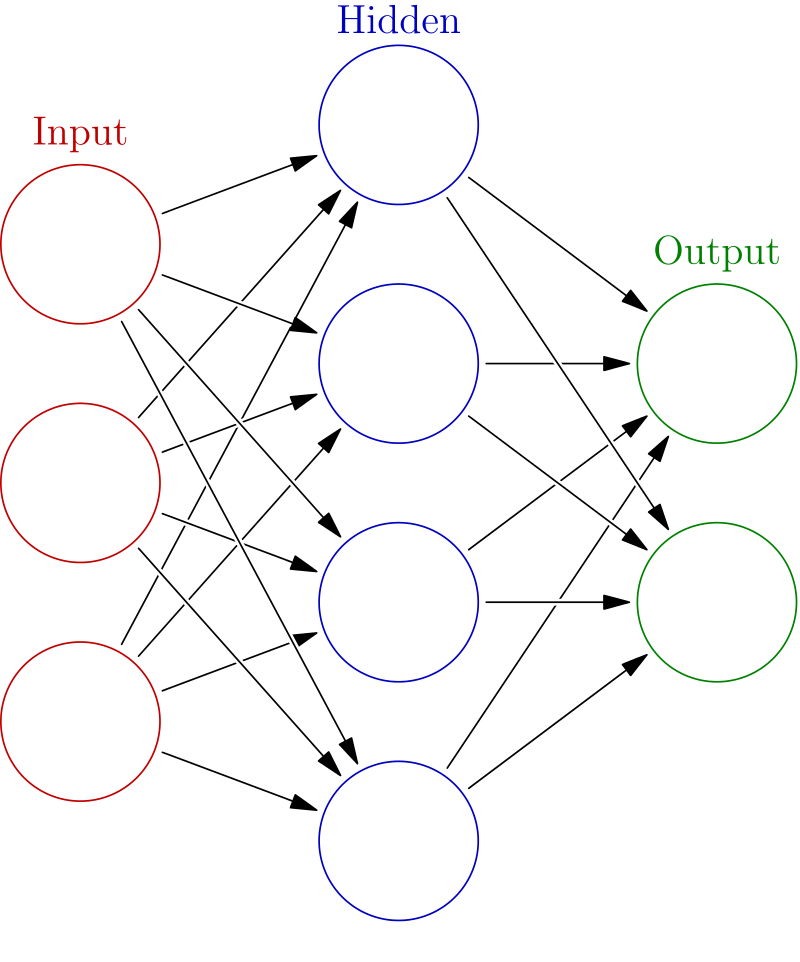
\includegraphics[width=0.5\linewidth]{images/neural}
	\caption{An example of a simple neural network.}
	\label{ip}
\end{figure}
Using this simple idea, many different species of neural networks may be constructed. The choices of network depth, number of connections, and activation function are examples of what are known as \textit{hyperparameters} which determine the behavior of the network.

\subsection{Convolutional Neural Networks}
\subsubsection{Convolutional Layer}
Vanilla ANNs usually connect each neuron in one layer to every other neuron in the preceding layer. This configuration is sufficient when the number of input neurons is small. However, as the number of input neurons increases (for example, as large as an image), the huge number of free parameters quickly leads to overfitting. Furthermore, the Vanilla ANN treats pixels with large spatial separation equally, which is often unnecessary for image processing where close spatial relationships are more important. \par Convolutional Neural Networks (CNNs) solve this problem by connecting only a small number of the input neurons (known as the receptive field) to the layers below, known as convolutional layers.
\begin{figure}[H]
	\centering
	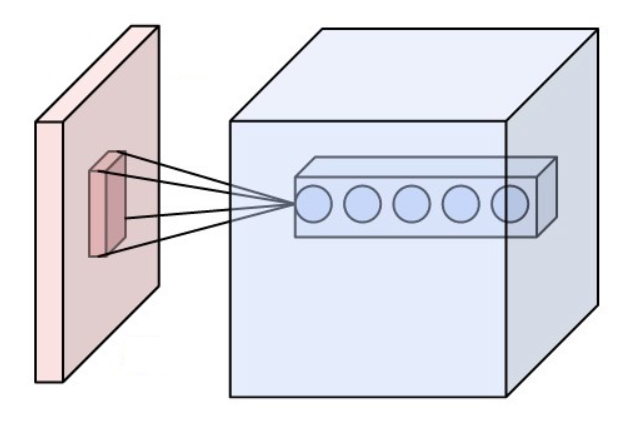
\includegraphics[width=0.5\linewidth]{images/Conv_layer}
	\caption{The red box represents the input neurons, with the receptive field connected to the next five convolutional layers.}
\end{figure}

\begin{figure}[H]    
  \centering
    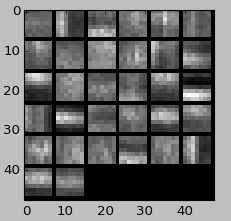
\includegraphics[width=0.5\linewidth]{images/ortho}
    \caption{Example of orthogonal filters in convolutional layer. NOTE: This is not from our network.}
    \label{ortho}
\end{figure}

The convolutional layer can be seen as a series of orthogonal filters, with each filter designed to identify a particular feature in an input image. An example of these orthogonal filters can be seen in Figure \ref{ortho}.Each filter size corresponds to the size of the receptive fields. The receptive fields overlap, so each filter is applied to every pixel in the input image. Weights are shared between each neuron in the filter so training time can be greatly reduced.
\subsubsection{Max Pooling Layer}
After each convolutional layer, the information is fed into a max pooling layer. This layer has the effect of increasing the non-linearity of the network, while also decreasing the amount of neurons to control overfitting. Max pooling layers divide up the output of the convolutional layer into zones, then selects the maximum value within each zone. This can be visualized using Figure \ref{pooling}.
\begin{figure}[H]
	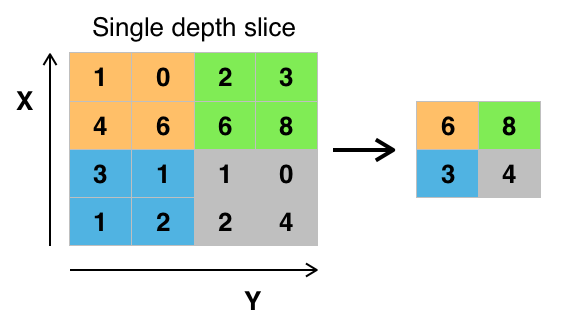
\includegraphics[width=\linewidth]{images/Max_pooling}
	\caption{Max pooling with a 2x2 kernel and a stride of 1.}
	\label{pooling}
\end{figure}
Max pooling layers may not be the right choice for the ideal network. Since the inversion problem is already ill-posed, layers that lose information such as the max pooling layer may not help the network converge on a solution. We have tested the current iteration of the  network both with and without max pooling layers and it didn't appear to change the accuracy or training time of the network; however training the network on more complicated datasets will determine the usefulness of the max pooling layer.
\subsubsection{Inner Product Layer}
After several iterations of convolutional and max pooling layers, the data is fed into an inner product layer, also known as a fully-connected layer. The neurons in this layer are connected to every neuron in the layer above, as in Figure \ref{ip}. This layer serves to provide high-level reasoning and logical capabilities to the network.
\subsubsection{ReLU Layer}
Between each inner product layer, we have a so-called Rectified Linear Unit (ReLU) layer. This layer adds further non-linearity to the decision making capacity of the network. The ReLU operation consists of applying the non-saturating activation function
\begin{equation}
f(x) = \max(0, x)
\end{equation} to each neuron in the layer. This layer has the added benefit of maintaining positivity, an important characteristic of solutions to the inversion problem.
\subsubsection{Loss Layer}
The loss layer drives the training of the network. The output of the last inner product layer (the proposed solution) is fed into the loss layer which is compared to the actual solution (known hereafter as \textit{truth}) to determine how well the network performed. This quantified using what is known as Euclidean loss, defined by
\begin{equation}
r(\mathbf{p},\mathbf{q}) = \frac{1}{2N} \sqrt{\sum_{i=0}^{N}(q_i - p_i)^2}.
\end{equation}
where $N$ is the number of output pixels, $p$ is the truth value and $q$ is the CNN outout value. This quantity is then used in the back-propogation phase of the training (explained below) to inform the network how it should adjust the weights.
\subsubsection{Forward/Backward Propogation}
Training the network involves two phases. The first phase, known as forward propagation, takes input and uses the neural network to compute the solution for that input. Forward propagation is used both for training the network and in the deployed network after it has been trained. This process is summarized in Figure \ref{forward}.
\begin{figure}[H]
	\centering
	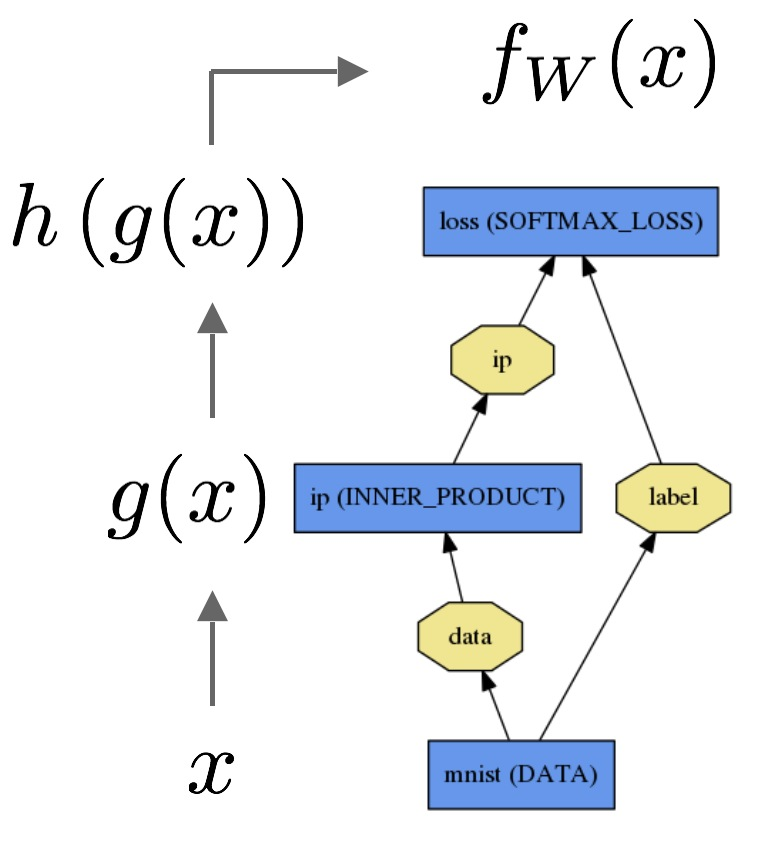
\includegraphics[width=0.6\linewidth]{images/forward}
	\caption{A basic neural network to demonstrate forward propogation. \cite{caffe}}
	\label{forward}
\end{figure}
The data $x$ is fed into an inner product layer $g(x)$ which is then given to a softmax layer (a common layer for classification problems) to form $h(g(x))$, which is ultimately provided to a softmax loss layer, which compares the proposed solution to the actual solution (often known as the \textit{label} in the literature). The final result is $f_W(x)$ where $W$ is a particular set of weights \cite{caffe}.
The second phase is termed backward propagation and is used only to train the network. It works by utilizing the gradient of the loss to construct an update to the weights. This process is demonstrated in Figure \ref{backward}.
\begin{figure}[H]
	\centering
	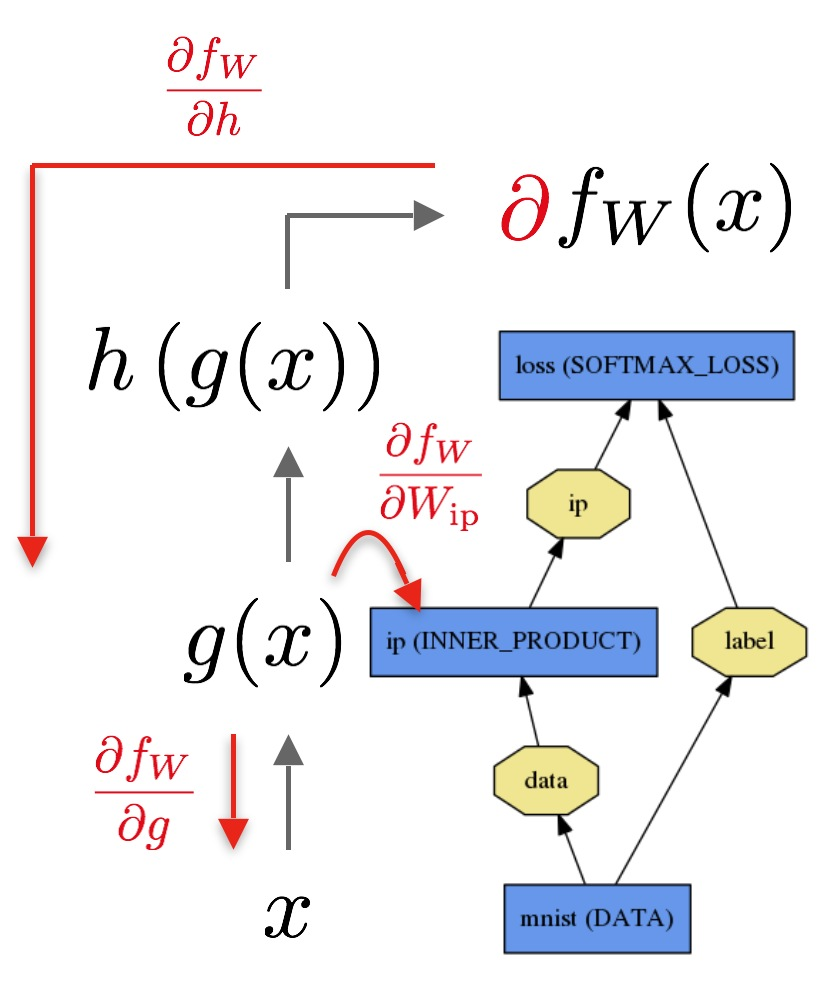
\includegraphics[width=0.6\linewidth]{images/backward}
	\caption{The same network as Figure \ref{forward} after applying backwards propogation.\cite{caffe}}
	\label{backward}
\end{figure}
The backward pass calculates the gradient of the loss with respect to the output $\frac{\partial f_W}{\partial h}$. The operation then continues to find the gradient with respect to each layer of the network using the chain rule, e.g. $\frac{\partial f_W}{\partial g}$. Furthermore, layers with input parameters, such as the inner product layer also compute the gradient with respect to their parameters, $\frac{\partial f_W}{\partial W_{ip}}$.

\subsubsection{Updating Weights}
To converge on a solution, the neural network must update thousands of weights in an attempt to decrease the average loss over the whole training dataset. Mathematically, we can describe the average loss $L(W)$ using the expression
\begin{equation}
L(W) = \frac{1}{|D|} \sum_{i}^{|D|} f_W(x_i) + \lambda r(W),
\end{equation}
where $f_W(x_i)$ is the loss on data instance $x_i$, $|D|$ is the set of all input data instances, and $r(W)$ is a regularization term incorporating the coefficient $\lambda$. This average loss is then used to update the weights. There are many different schemes for updating the weights, the one we selected is known as \textit{Stochastic Gradient Descent} (SGD). It calculates the \textit{update value} $V_{t+1}$ and the updated weights $W_{t+1}$ using from the previous iteration $t$ the recursion relations
\begin{align}
V_{t+1} &= \mu V_t - \alpha_t \nabla L(W_t)
\intertext{and}
W_{t+1} &= W_t + V_{t+1},
\end{align}
where $V_t$ is the previous update value, $W_t$ is the set previous weights, $\alpha_t$ is the learning rate, and $\mu$ is the momentum. \par As the learning rate starts to plateau, it is often helpful to reduce the learning rate to converge on the solution.
For our network we chose an \textit{inverse decay} paradigm which is defined by
\begin{equation}
\alpha_t = \alpha_0 (1 + \gamma t)^{-\beta}
\end{equation}
where $\alpha_0$ (the base learning rate), $\gamma$, and $\beta$ are constant parameters provided to the network by the user.

\section{Software}
\subsection{Caffe}
To expedite the development process, we have taken advantage of a program called \textit{Caffe}, an open-source implementation of a convolutional neural network. Caffe allows the user to define a neural network using a script, and then trains the network using provided input and truth datasets. \par The developers of Caffe have reduced the CNN algorithm to a sequence of matrix multiplication. This allows computations using the \textit{Basic Linear Algebra Subprograms} (BLAS) routines, highly optimized programs that have been implemented on many different architectures. This generalization means that Caffe can be run on a graphics processing unit (GPU) to greatly accelerate training time through the GPU's impressive floating-point performance. \par This program also includes an API which allows development of custom code that can access the network and use the output in other routines.
\subsection{Custom Routines}
All routines that were used to generate the datasets and validate the network were programmed in C++. This language choice allowed easy access to the Caffe API (which was also implemented in C++), and the benefits of decreased runtime for large dataset manipulation.

\section{Testing CNNs Using Simulated Data}
\subsection{Introduction}
To help us learn how to use CNNs, we solved two simple cases of the MOSES inversion problem: 4x4 pixel input/output image with one pixel greater than zero, all other pixels zero and a 8x8 pixel input/output image with five pixels greater than zero. Using simple cases allowed us to build and debug the network without having to deal with large, complicated real datasets.
\subsection{Dataset Preparation}
The MOSES instrument observes the sun in spatial directions $x$ and $y$. This measurement is the projection of a spectral cube in $x$, $y$, and $\lambda$. In the MOSES coordinate system $x$ is the dispersion direction. Therefore, if we neglect the point-spread function, we may ignore the $y$ component of the images without loss of generality. \par For this test we randomly construct a slice of the spectral cube with dimensions $x$ and $\lambda$. This is the truth image, and the output of the neural network should strive to create this output. 
\begin{figure}[H]  
	\centering
	 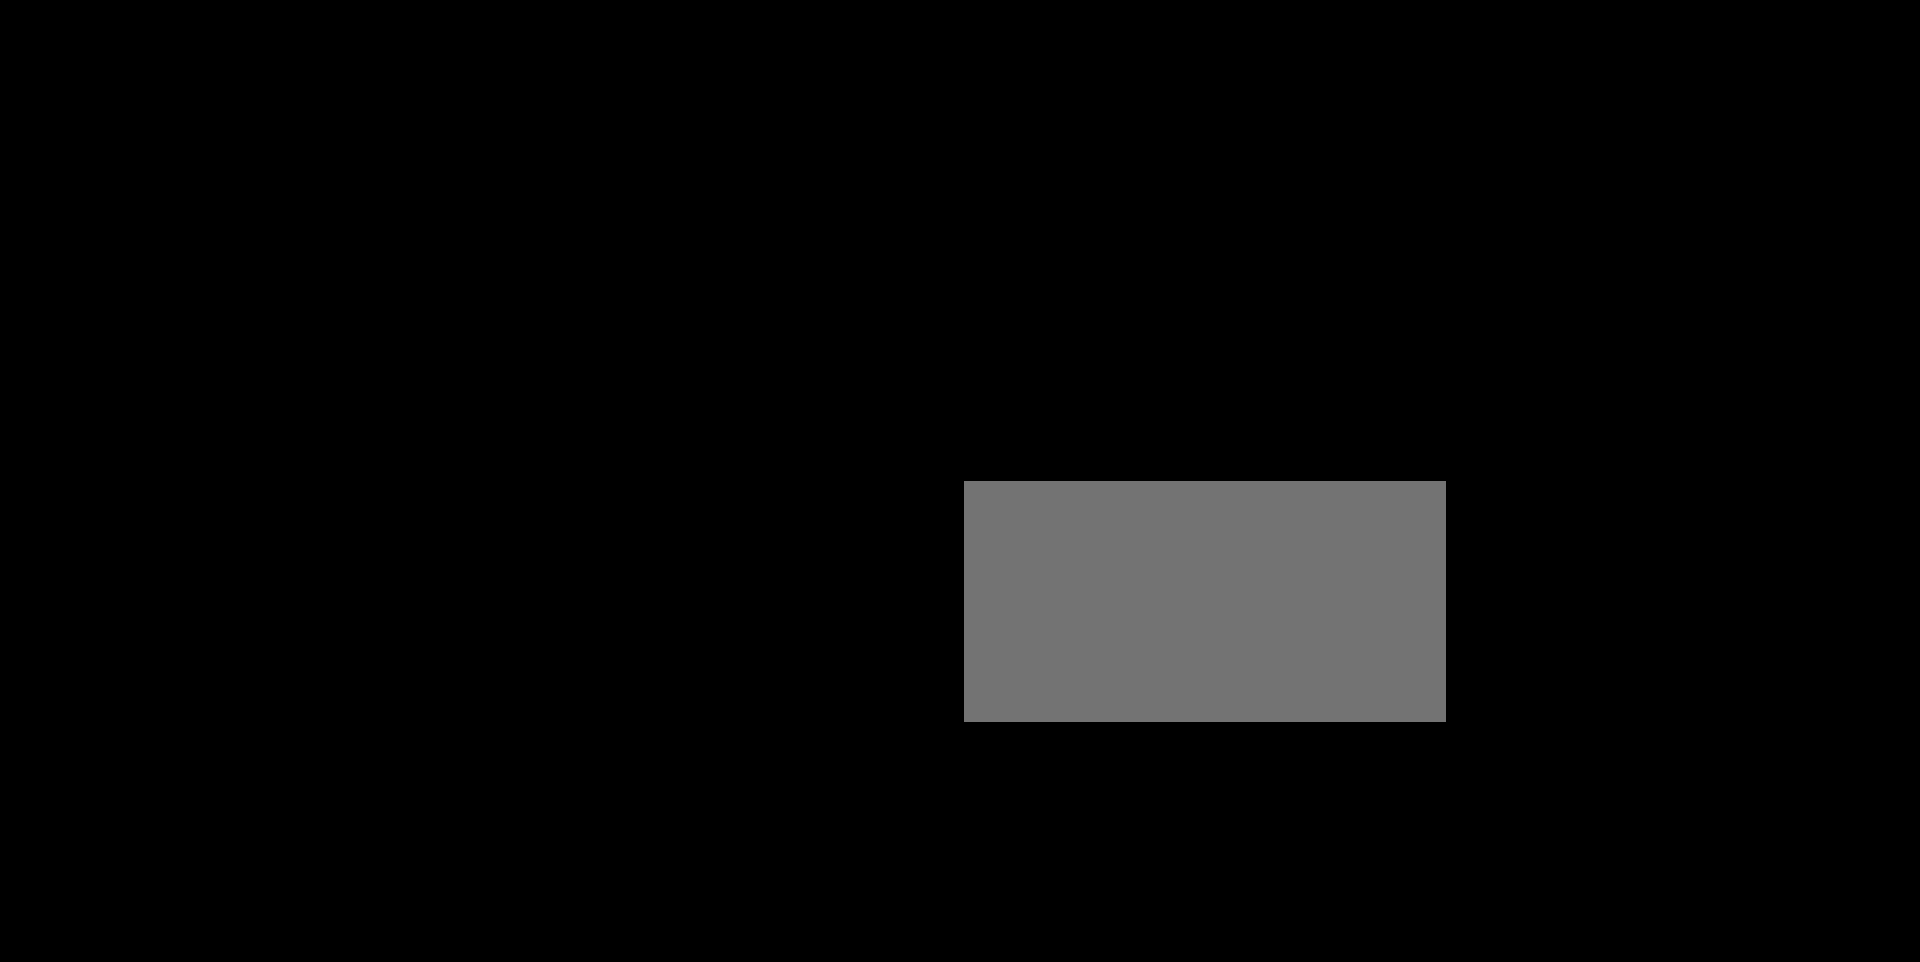
\includegraphics[width=0.75\linewidth]{images/mIn}
	 \caption{An example of a 4x4 pixel truth image. For this image and all following images, the vertical axis is $\lambda$ and the horizontal axis is $x$.}
	 \label{mIn}
\end{figure}
From the truth image, we simulate the measurements captured by the instrument using the MOSES forward model. The forward model works by summing along each spectral direction (as described in Figure \ref{inversion}) for the $m=0$, $1$, and $-1$ spectral orders. Since the $y$ dimension has been ignored, we are left with a graph, described in Figure \ref{m1-1}
 
 \begin{figure*}
     \centering
     \begin{subfigure}[b]{0.3\textwidth}
         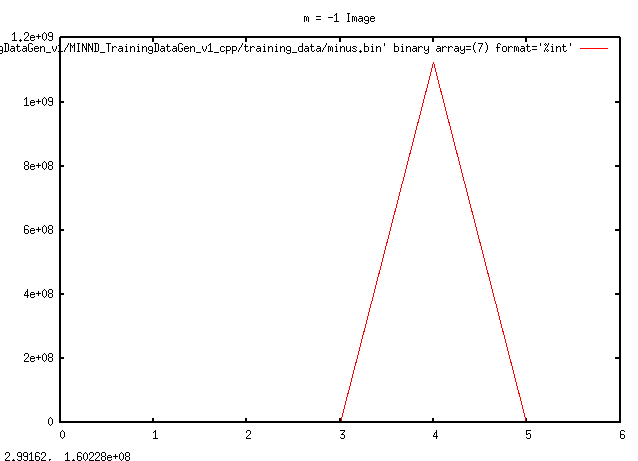
\includegraphics[width=\textwidth]{images/m-1}
         \caption{$m = -1$ order }
     \end{subfigure}
      \begin{subfigure}[b]{0.3\textwidth}
          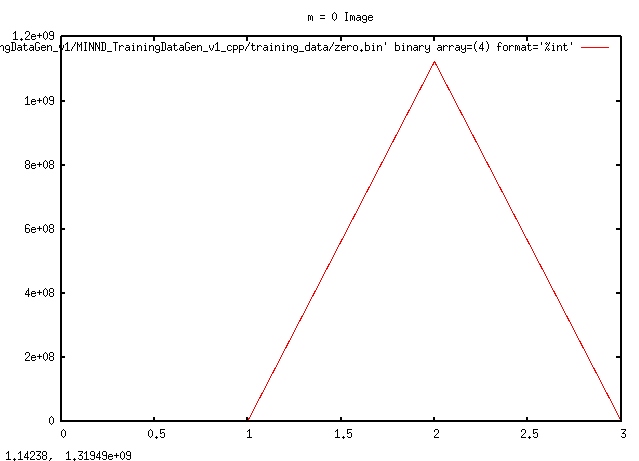
\includegraphics[width=\textwidth]{images/m0}
          \caption{$m = 0$ order }
      \end{subfigure}
        \begin{subfigure}[b]{0.3\textwidth}
            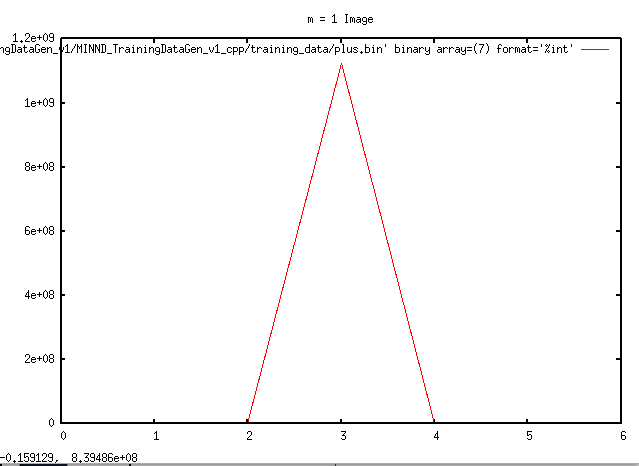
\includegraphics[width=\textwidth]{images/m1}
            \caption{$m = 1$ order }
        \end{subfigure}
 
     \caption{Simulated results of the MOSES instrument for the simple case described in Figure \ref{mIn}.}
     \label{m1-1}
 \end{figure*}

\begin{figure}[H]   
	\centering
	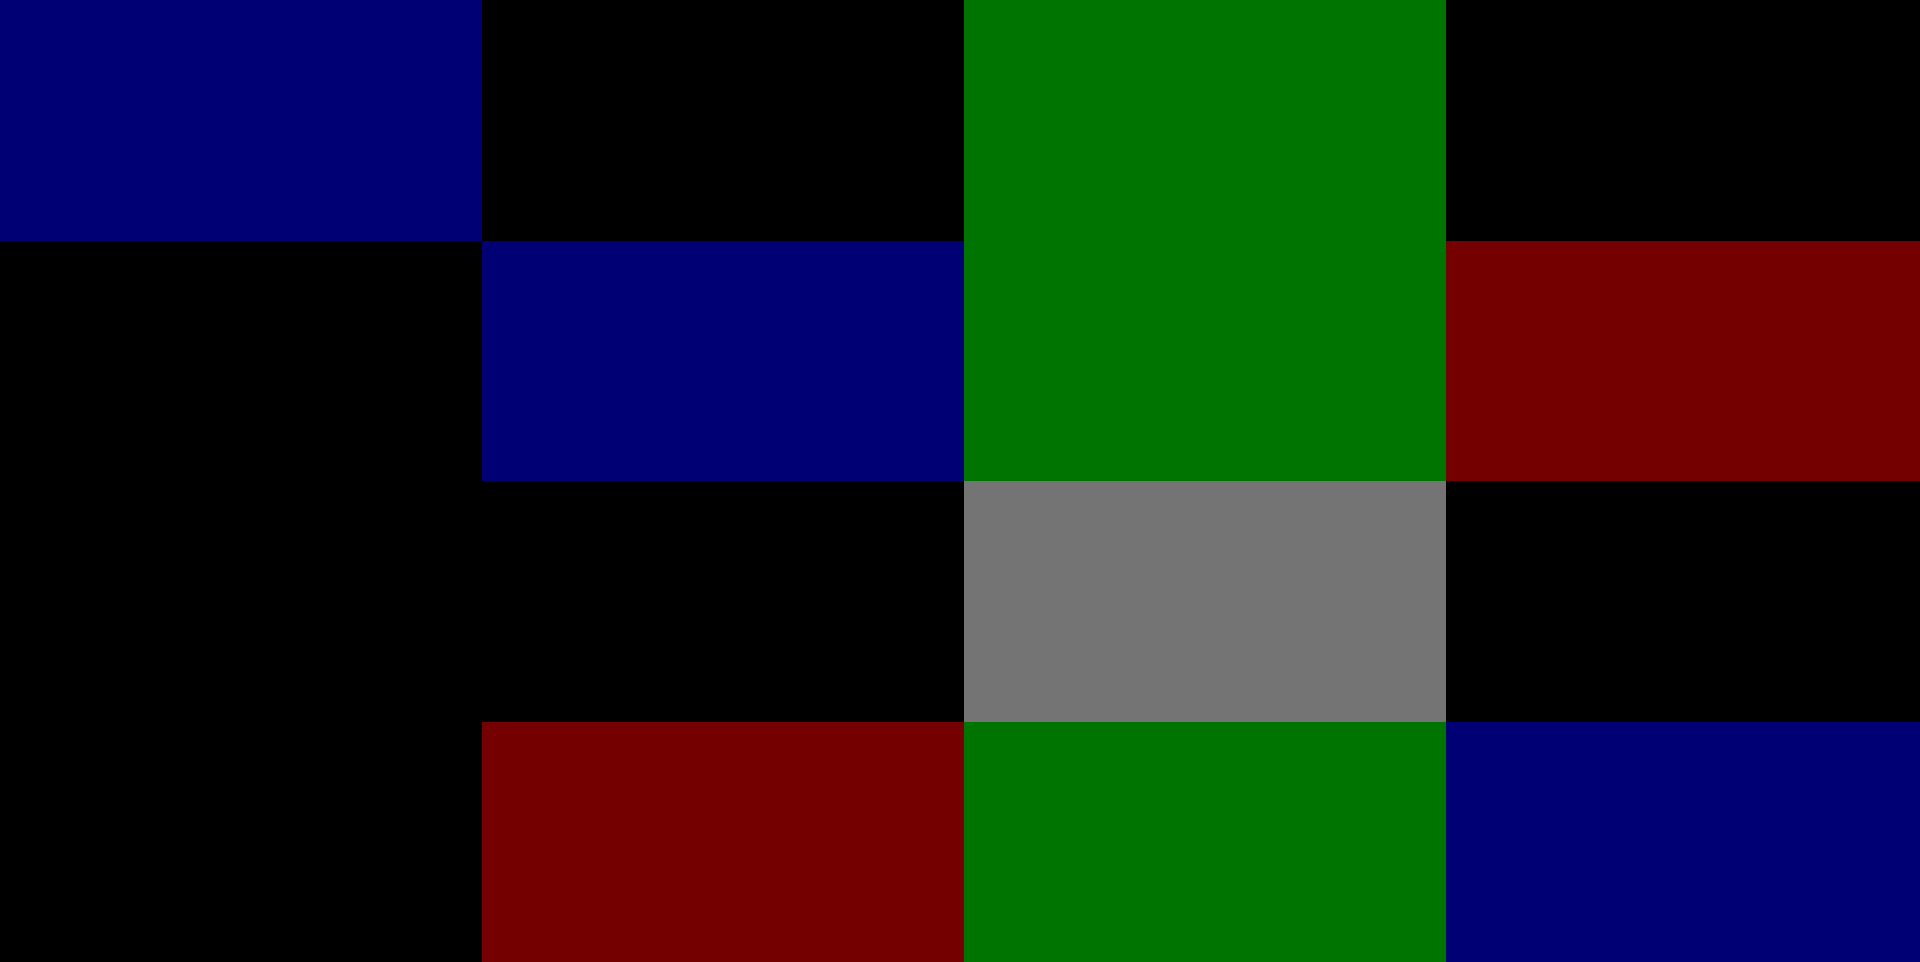
\includegraphics[width=0.75\linewidth]{images/mOut}
	\caption{An example of a 4 pixel by 4 pixel input image.}
	\label{mOut}
\end{figure}

We can speed up the training time of the neural network by providing it some information about how the MOSES forward model works. To do this, we transform the graphs from the three orders back into an image by back-projecting along each spectral direction. The result is essentially an image that contains the maximum possible pixel value at every location in the spectral slice. For our purposes we will store the projections from each order on separate color channels (RGB). We will call this image the \textit{input} image, as it is fed into the neural network. An example of this image is given in Figure \ref{mOut}.
\subsection{Results}
\subsubsection{One Active Pixel}
The learning and input parameters of the one active pixel network are summarized in Table \ref{4x4tab}. Unfortunately the image depth is not very large, it is a result of creating a simple database of bitmap images for the CNN's input and truth dataset. \par The topography of our first neural network was based off of Google's LeNET image classification neural network, described in Figure \ref{4x4net}. It consists of one convolutional layer, one max pooling layer, and three inner product layers with ReLU layers in between. \par This network performed very well, according to the loss. We can see visually in Table \ref{4x4tab} that the output image is very close to the truth image. Since the training dataset (10,000) is larger than the number of possible images $4 \times 4 \times 256 = 4096$, it likely that the neural network simply memorized the training dataset.

\subsubsection{Five Active Pixels}

The input parameters for the five-active-pixel case are cataloged in the second column of Table \ref{4x4tab}.  They are very similar to the case above, with the exception of the base learning rate $\alpha_0$ which was reduced to account for the longer training time. \par The five-active-pixel case is a much harder problem than the one-pixel case, therefore the solutions posed by the neural network aren't perfect matches to truth. However in looking at the results displayed in Table \ref{8x8im} we can see that the many of the brightest pixels in the output and truth images match. \par This behavior is encouraging since this problem is potentially harder than the actual MOSES inversion problem. This is because the data is arranged randomly in space, and there are no solar features to be identified by the network. It is troubling that the images produced by the network aren't always solutions to the MOSES inversion problem. Perhaps the network could be better constrained to ensure all output is a valid solution to the inversion problem.

\begin{table*}
\centering
\begin{tabular}{|l|c|c|}
\hline
Quantity & One Active Pixel & Five Active Pixels \\ \hline
$\alpha_0$ & 0.1 & 0.01\\ \hline
$\gamma$ & 0.0001 & 0.0001\\ \hline
$\beta$ & 0.75 & 0.75 \\ \hline
$\mu$ & 0.9 & 0.9\\ \hline
$x$ & 4 pixels & 8 pixels\\ \hline
$\lambda$  & 4 pixels & 8 pixels\\ \hline
Image depth & 8 bits & 8 bits\\ \hline
Intensity range & $[0,1]$  & $[0,1]$\\ \hline
Training dataset & $10^4$ images & $10^6$ images\\ \hline
Training time &  5 minutes & 60 minutes\\ \hline
Loss & $5.385\times10^{-5}$ & 0.127\\ \hline
\end{tabular}
\caption{Parameters describing the CNN used to train the one active pixel case}
\label{4x4tab}
\end{table*}
\begin{figure*}
\centering
\begin{subfigure}[b]{0.42\textwidth}  
	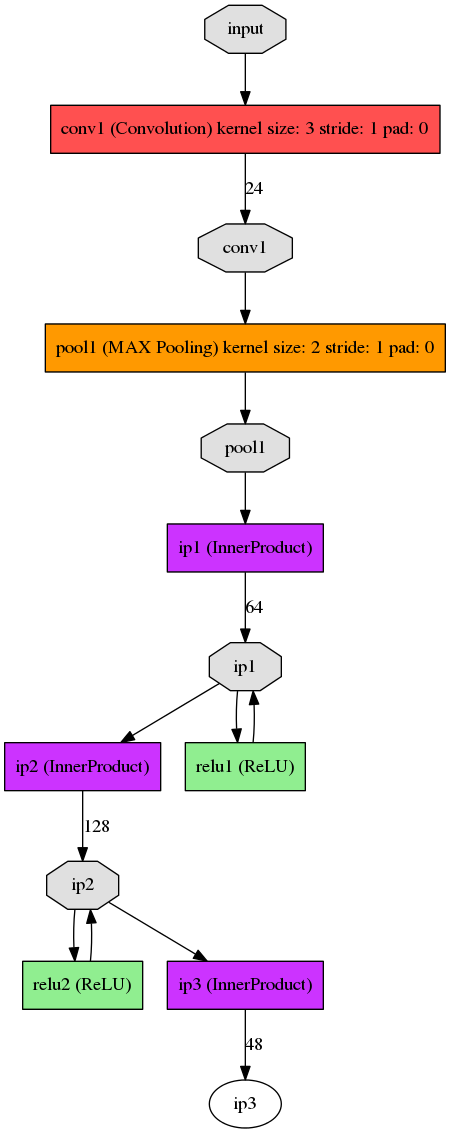
\includegraphics[width=0.9\textwidth]{images/4x4/minnd_dia_4x4}
	\caption{Topography of the our CNN for the one active pixel case}
	\label{4x4net}
\end{subfigure}
\begin{subfigure}[b]{0.42\textwidth}
	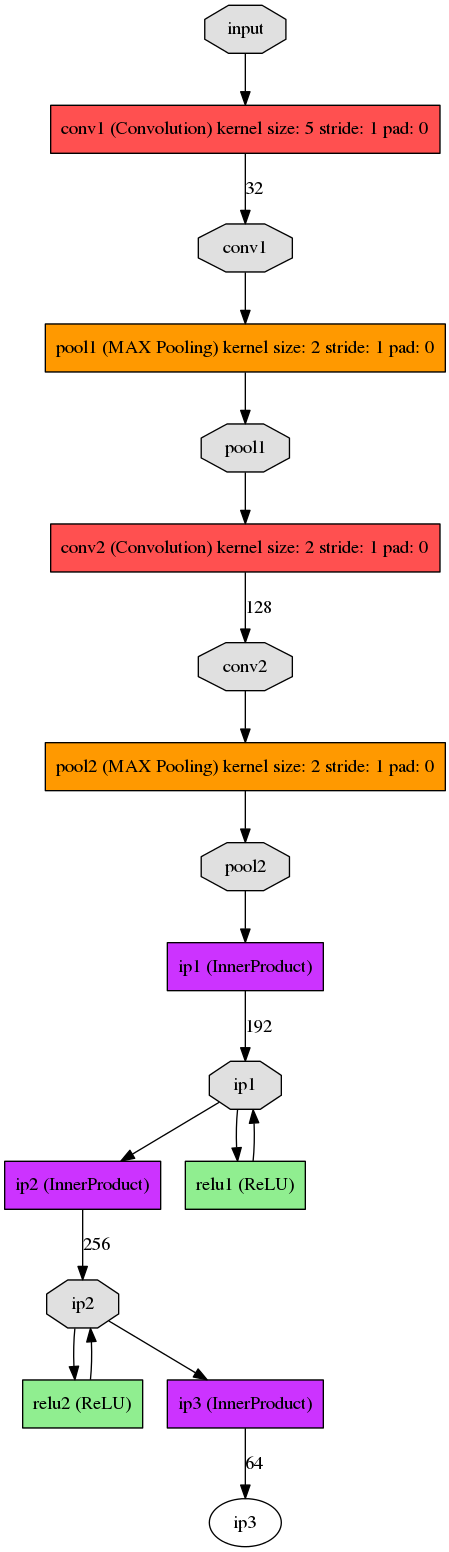
\includegraphics[width=0.9\textwidth]{images/8x8/minnd_dia}
	\caption{Topography of the our CNN for the five active pixels case}
	\label{8x8net}
\end{subfigure}
\caption{Topography of the two neural networks used in the test.}
\end{figure*}

\begin{table*}
\begin{tabular}{| r | c | c | c | c |}
\hline
Iteration & Input & Output & Truth & Difference \\ \hline
1 & 
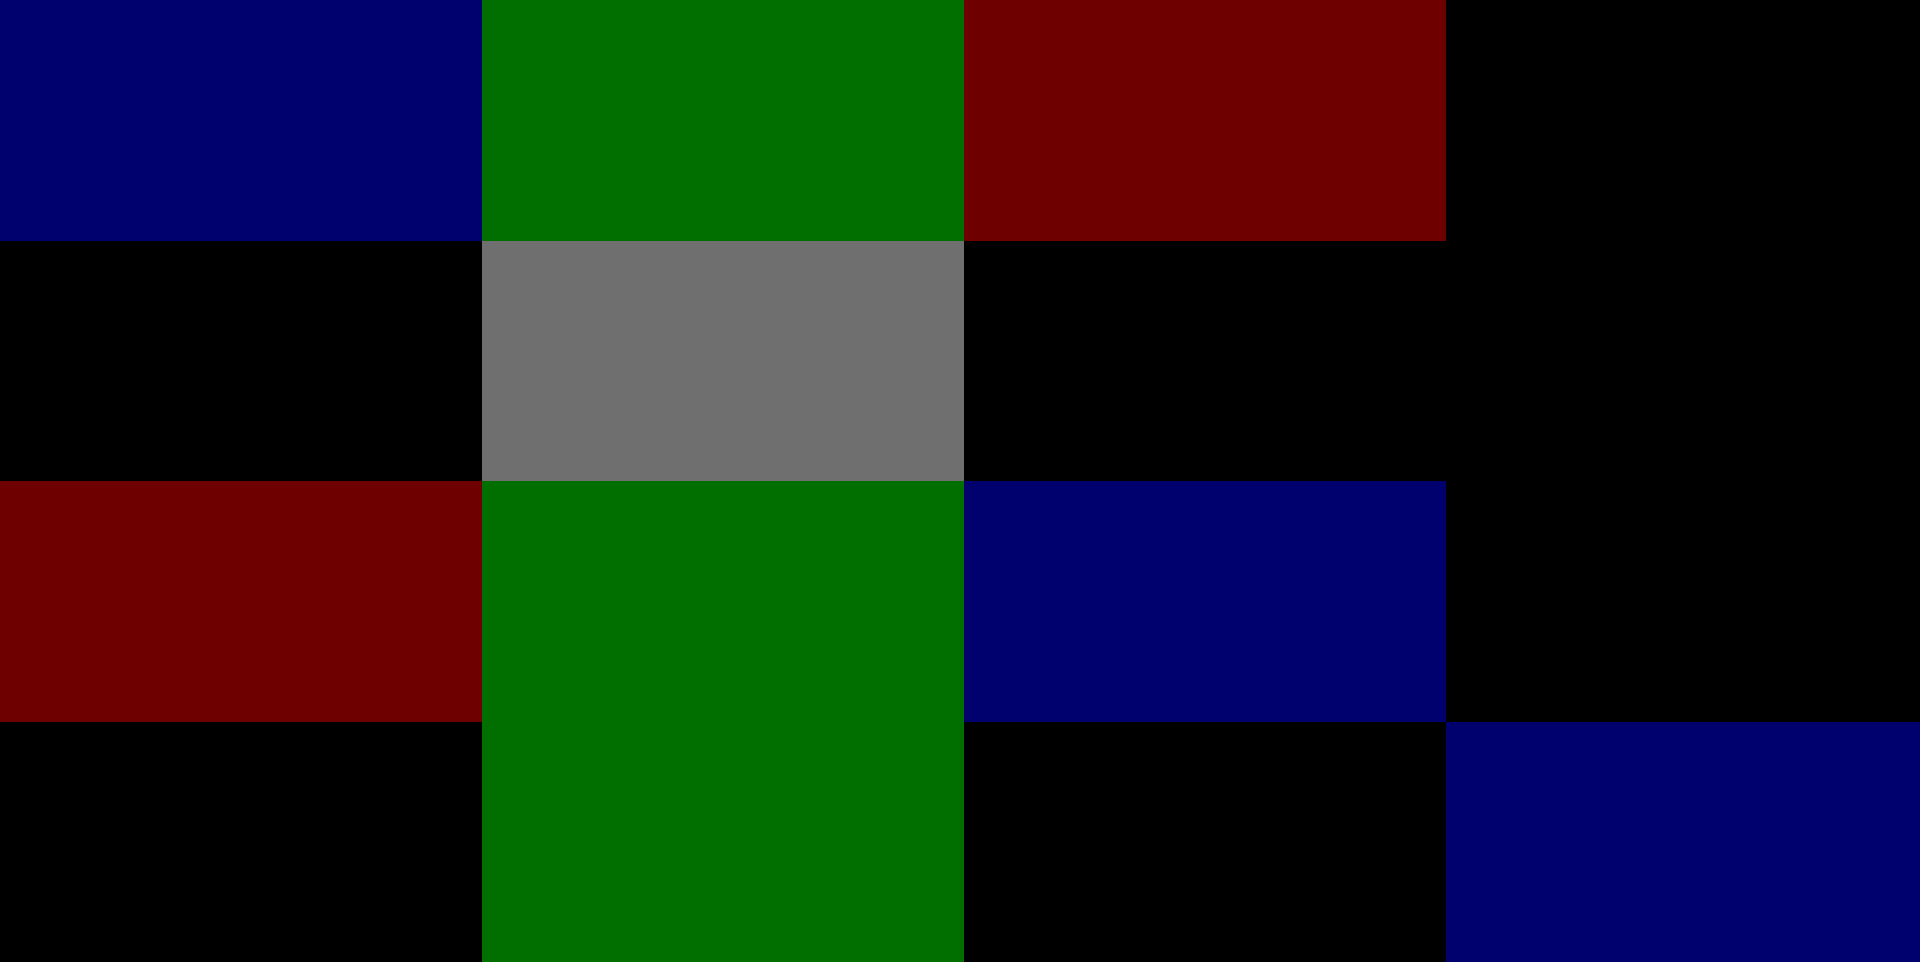
\includegraphics[width=0.2\textwidth]{images/4x4/1/in} &

\includegraphics[width=0.2\textwidth]{images/4x4/1/out} &
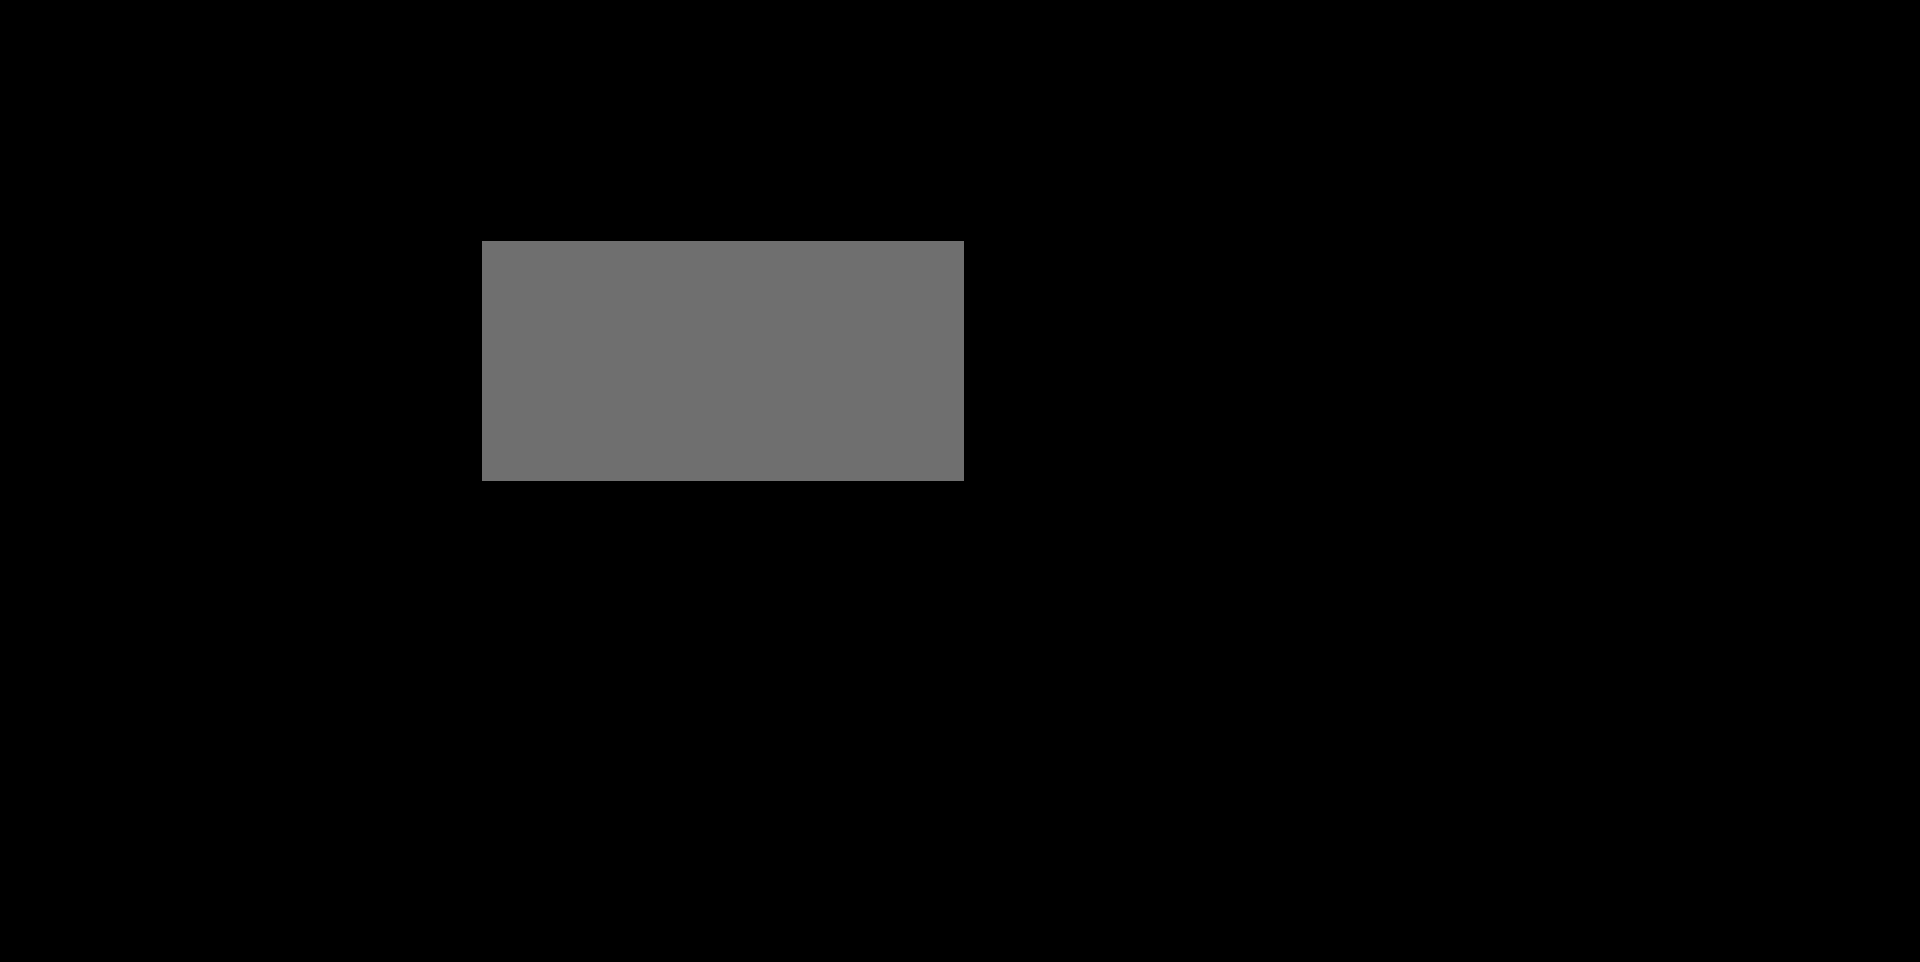
\includegraphics[width=0.2\textwidth]{images/4x4/1/truth} &

\includegraphics[width=0.2\textwidth]{images/4x4/1/dif} \\ \hline
\end{tabular}
\caption{Characteristic output for the 4x4 case. MINND performs perfectly each time.}
\end{table*}

\begin{table*}
\begin{tabular}{| r | c | c | c | c |}
\hline
Iteration & Input & Output & Truth & Difference \\ \hline
1 & 
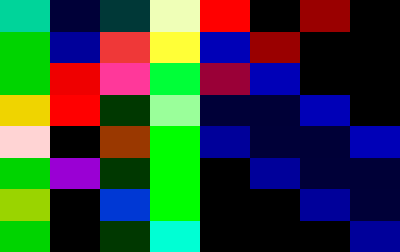
\includegraphics[width=0.2\textwidth]{images/8x8/1/in} &

\includegraphics[width=0.2\textwidth]{images/8x8/1/out} &
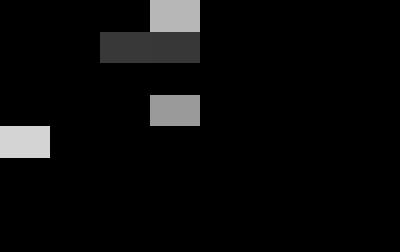
\includegraphics[width=0.2\textwidth]{images/8x8/1/truth} &

\includegraphics[width=0.2\textwidth]{images/8x8/1/dif} \\ \hline
2 & 
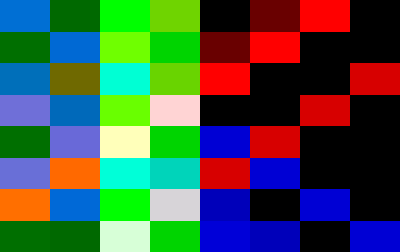
\includegraphics[width=0.2\textwidth]{images/8x8/2/in} &

\includegraphics[width=0.2\textwidth]{images/8x8/2/out} &
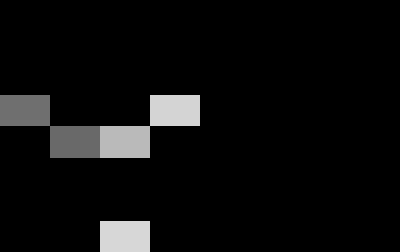
\includegraphics[width=0.2\textwidth]{images/8x8/2/truth} &

\includegraphics[width=0.2\textwidth]{images/8x8/2/dif} \\ \hline
3 & 
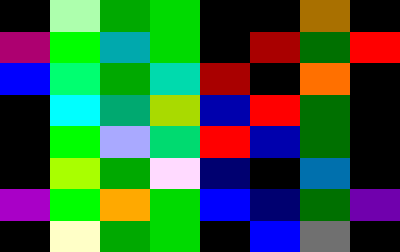
\includegraphics[width=0.2\textwidth]{images/8x8/3/in} &

\includegraphics[width=0.2\textwidth]{images/8x8/3/out} &
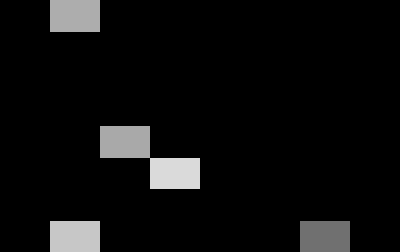
\includegraphics[width=0.2\textwidth]{images/8x8/3/truth} &

\includegraphics[width=0.2\textwidth]{images/8x8/3/dif} \\ \hline
4 & 
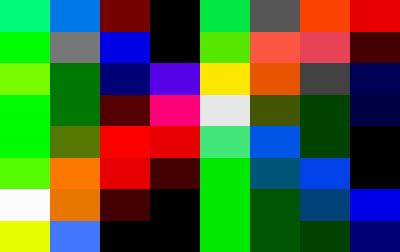
\includegraphics[width=0.2\textwidth]{images/8x8/4/in} &

\includegraphics[width=0.2\textwidth]{images/8x8/4/out} &
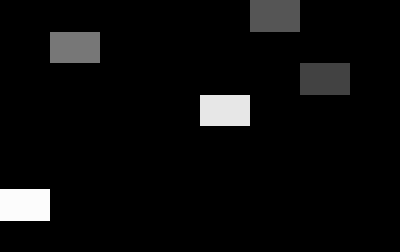
\includegraphics[width=0.2\textwidth]{images/8x8/4/truth} &

\includegraphics[width=0.2\textwidth]{images/8x8/4/dif} \\ \hline
\end{tabular}
\caption{Output of the MINND neural network for four randomly selected input images. Notice how not all output images are solutions to the inversion problem.}
\label{8x8im}
\end{table*}

\section{Conclusion}

We have showed that a convolutional neural network may be a viable option for MOSES data inversion. 8 by 8 pixel able to be reasonably inverted by the neural network. \par Possible improvements include: enforcing neural network output to make the output a solution to the inversion problem, modifying the hyperparameters of the network, and a better database for managing larger image sets. \par Next we hope to apply convolutional neural networks to the IRIS dataset. This will allow us to analyze the performance on solar data, and allow us to perform inversions on the MOSES dataset.





\end{multicols}

	%\bibliographystyle{apj}
	\bibliographystyle{unsrt}
	\bibliography{sources}
\end{document}
